\title{%
  Variabler och funktioner
}
\author{Daniel Bosk}
\institute{%
  KTH EECS
}

\mode<article>{\maketitle}
\mode<presentation>{%
  \begin{frame}
    \maketitle
  \end{frame}
}

\mode*

\begin{abstract}
  % What's the problem?
% Why is it a problem? Research gap left by other approaches?
% Why is it important? Why care?
% What's the approach? How to solve the problem?
% What's the findings? How was it evaluated, what are the results, limitations, 
% what remains to be done?

% XXX Summary
\emph{Summary:}
\dots

% XXX Motivation and intended learning outcomes
\emph{Intended learning outcomes:}
\dots

% XXX Prerequisites
\emph{Prerequisites:}
\dots

% XXX Reading material
\emph{Reading:}
\dots

\end{abstract}


\section{Programmering}

\subsection{Vad är programmering?}

\begin{frame}
  \begin{block}{Dator}
    \begin{itemize}
      \item Processor
      \item Minne
      \item Annan hårdvara
    \end{itemize}
  \end{block}
\end{frame}

\begin{frame}
  \begin{block}{Processorn}
    \begin{itemize}
      \item Exekverar maskinkod --- program
    \end{itemize}
  \end{block}

  \pause

  \begin{example}
    \begin{itemize}
      \item<1-2> 00012000050000020500
      \item<3-> 0001 2000 0500
      \item<3-> 0002 0500
    \end{itemize}
  \end{example}
\end{frame}

\begin{frame}
  \begin{block}{Svar}
    \begin{itemize}
      \item Programmering är att skriva program.
    \end{itemize}
  \end{block}
\end{frame}


\subsection{Programmeringsspråk}

\begin{frame}
  \begin{block}{Programmeringsspråk}
    \begin{itemize}
      \item Ett språk för människor att skriva datorprogram.
    \end{itemize}
  \end{block}
\end{frame}

\begin{frame}[fragile]
  \begin{example}[Python]
    \begin{minted}{python}
print("Hello, World!")
    \end{minted}
  \end{example}

  \pause

  \begin{example}[C++]
    \begin{minted}{c++}
#include <iostream>
using namespace std;

int main(void) {
    std::cout << "Hello, World!" << std::endl;
    return 0;
}
    \end{minted}
  \end{example}
\end{frame}

\begin{frame}
  \begin{remark}
    \begin{itemize}
      \item Måste översättas till maskinkod!
    \end{itemize}
  \end{remark}
\end{frame}


\section{Köra Python}

\subsection{Terminalen}

\begin{frame}
  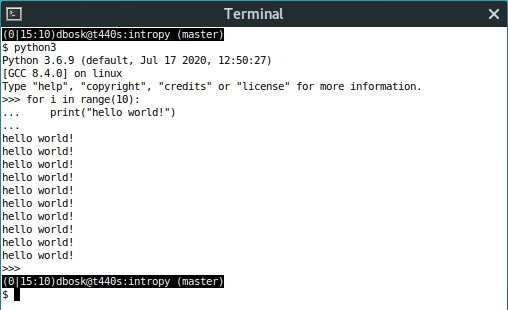
\includegraphics[width=\columnwidth]{figs/python-terminal.png}
\end{frame}


\subsection{Andra gränssnitt}

\begin{frame}
  \centering
  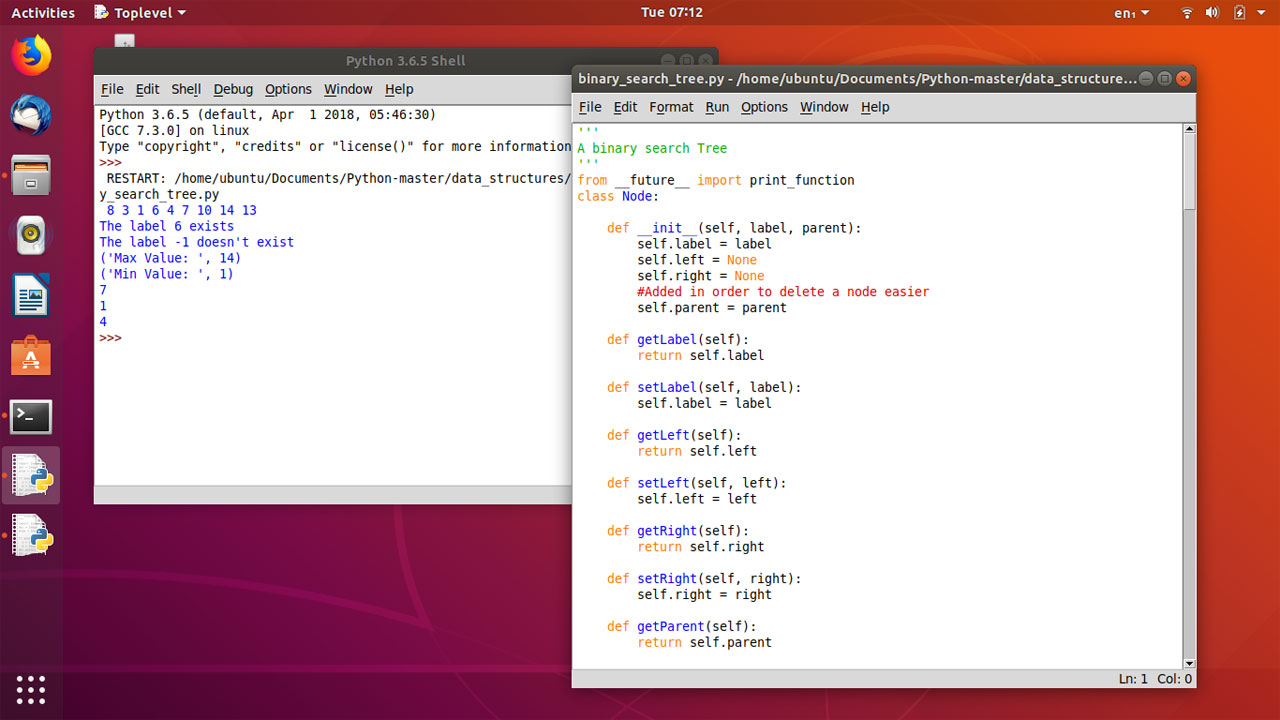
\includegraphics[width=\columnwidth]{figs/idle.jpg}
\end{frame}

\begin{frame}
  \centering
  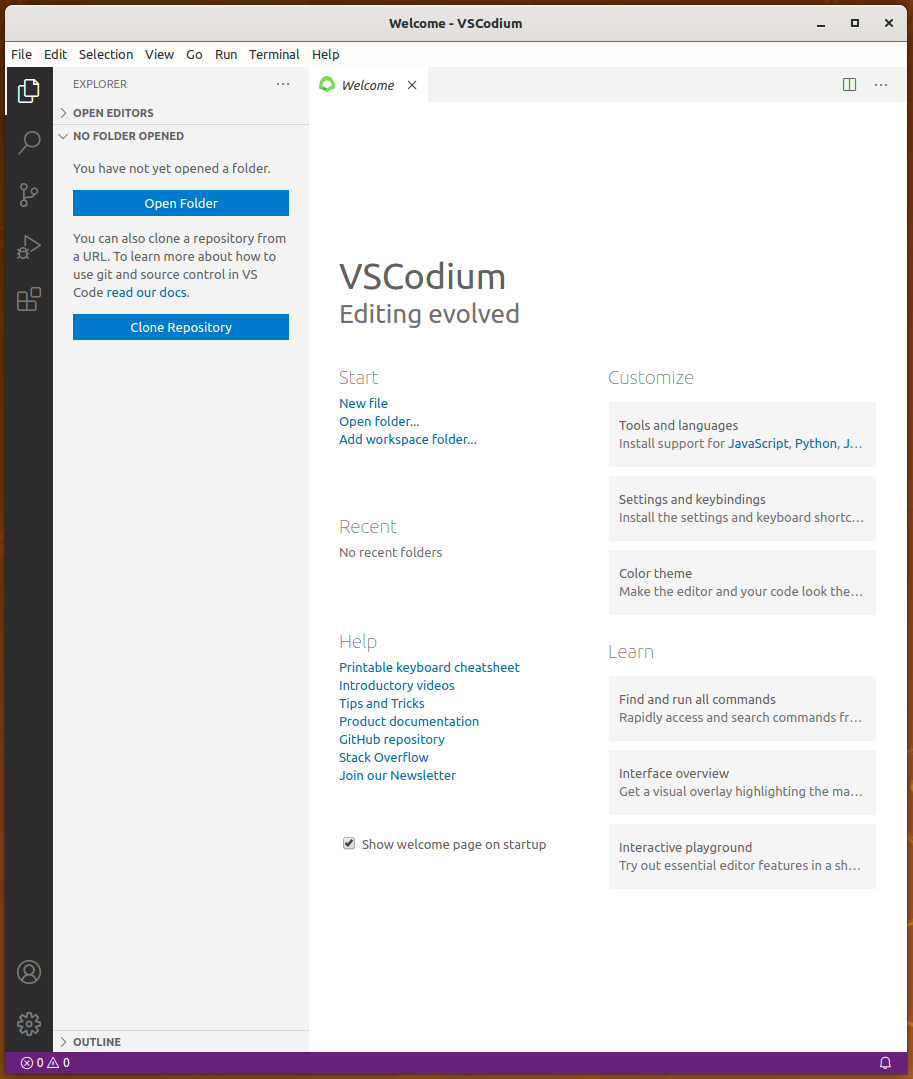
\includegraphics[height=\textheight]{figs/codium.png}
\end{frame}

\begin{frame}
  \centering
  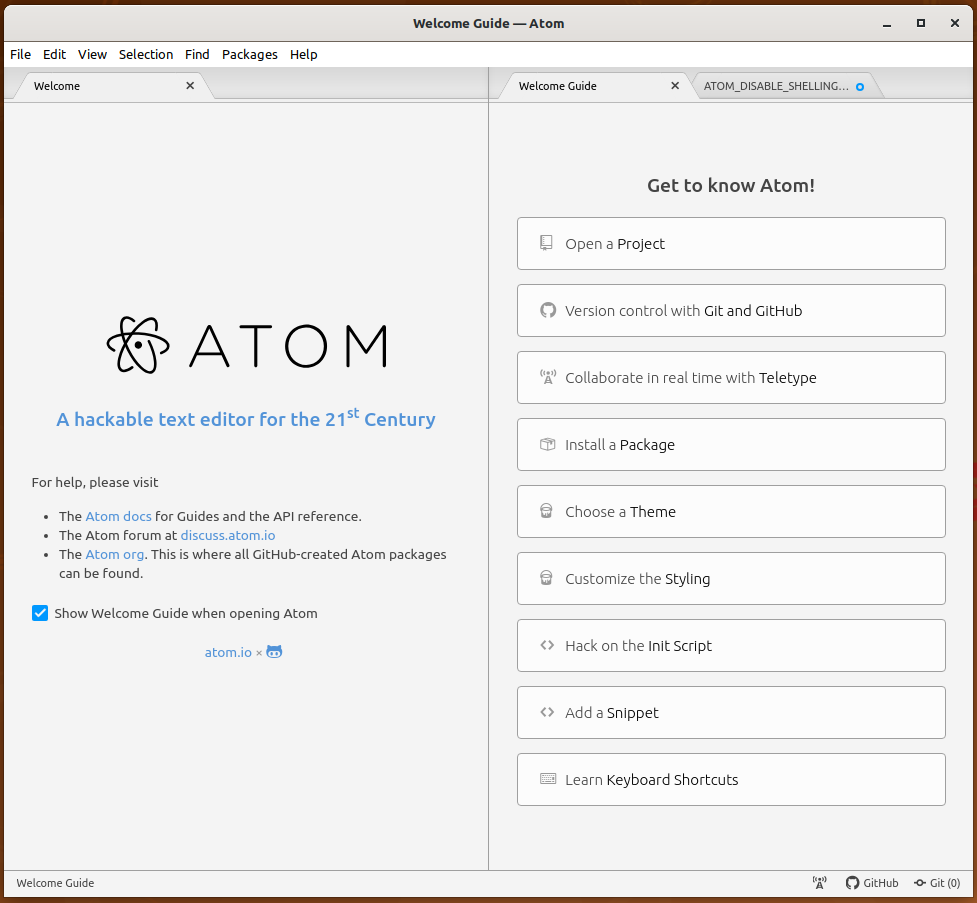
\includegraphics[height=\textheight]{figs/atom.png}
\end{frame}

\begin{frame}
  \centering
  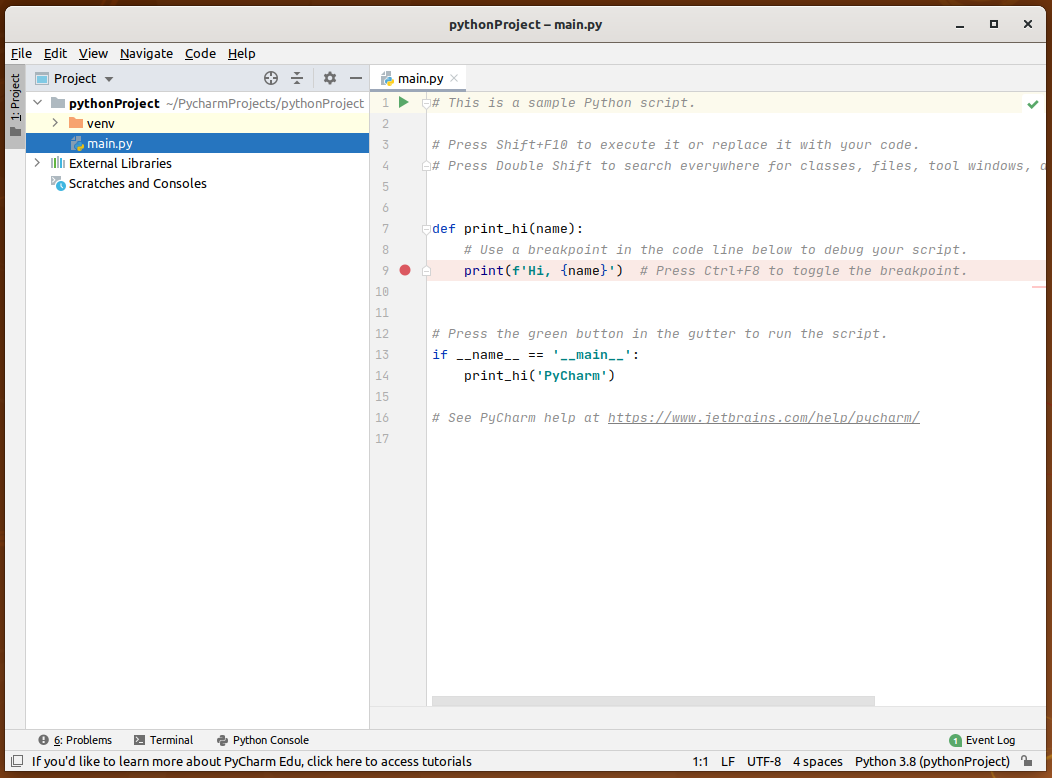
\includegraphics[height=\textheight]{figs/pycharm.png}
\end{frame}


\section{Skriva Pythonprogram}

\subsection{Kommentarer}

\begin{frame}
  \begin{center}
    \huge\#
  \end{center}
\end{frame}

\begin{frame}[fragile]
  \begin{example}
    \begin{minted}{python}
# Har kan vi skriva for manniskor.
# Python kommer att ignorera allt detta.
    \end{minted}
  \end{example}
\end{frame}

\begin{frame}[fragile]
  \begin{example}
    \begin{minted}{python}
"""
Detta ar dock lite enklare,
iallafall nar vi ska skriva pa flera
rader
"""
    \end{minted}
  \end{example}
\end{frame}


\subsection{Utskrifter}

\begin{frame}[fragile]
  \begin{block}{Funktionen \mint{python}|print|}
    \begin{itemize}
      \item Skriver ut sina argument till skärmen.
    \end{itemize}
  \end{block}

  \pause

  \begin{example}
    \begin{minted}{python}
# Skriver ut till skarmen
print("Hello, World!")
    \end{minted}
  \end{example}
\end{frame}


\subsection{Variabler och datatyper}

\begin{frame}
  \begin{block}{Data}
    \begin{itemize}
      \item Program är inte intressanta utan data.
      \item Data är av olika typer.
      \item Det går att göra olika saker med olika typer av data.
    \end{itemize}
  \end{block}

  \pause

  \begin{example}[Litteraler]
    \begin{itemize}
      \item "Hello, World!"
      \item 5
      \item 3.14
      \item True
    \end{itemize}
  \end{example}
\end{frame}

\begin{frame}[fragile]
  \begin{block}{Variabler}
    \begin{itemize}
      \item Identifierare.
      \item Hänvisar till minne där data finns lagrat.
      \item Håller koll på datatyp.
    \end{itemize}
  \end{block}

  \pause

  \begin{example}[Variabler]
    \begin{minted}{python}
x = 5
y = 2
name = "Daniel"
    \end{minted}
  \end{example}
\end{frame}

\begin{frame}
  \begin{remark}
    \begin{itemize}
      \item Får inte börja med en siffra.
      \item x är inte samma som X.
    \end{itemize}
  \end{remark}
\end{frame}

\begin{frame}[fragile]
  \begin{example}[Heltalsoperationer]
    \begin{minted}{python}
x = 4+1
y = 2
z = x * y
x2 = z / y
    \end{minted}
  \end{example}
\end{frame}

\begin{frame}[fragile]
  \begin{example}[Fler heltalsoperationer]
    \begin{minted}{python}
x = 5
y = x / 2
z = x // 2
xx = x**2
    \end{minted}
  \end{example}
\end{frame}

\begin{frame}[fragile]
  \begin{remark}
    \begin{itemize}
      \item \mint{python}|print| behöver datatypen sträng.
      \item Finns typkonvertering.
    \end{itemize}
  \end{remark}

  \begin{example}
    \begin{minted}{python}
name = "Daniel"
x = 5
print("Hej " + name + "!")
print(x)
    \end{minted}
  \end{example}
\end{frame}

\begin{frame}[fragile]
  \begin{example}
    \begin{minted}{python}
print("Ar " + x " stort?")
print("Ar " + str(x) + " stort?")
print("Ar {} stort?".format(x))
print(f"Ar {x} stort?")
    \end{minted}
  \end{example}
\end{frame}


\subsection{Konstanter}

\begin{frame}
  \begin{remark}[Konstanter varierar inte]
    \begin{itemize}
      \item Vissa språk förhindrar ändring av konstanter.
      \item Python har bara konvention.
      \item \mint{python}|PI = 3.14|
    \end{itemize}
  \end{remark}
\end{frame}


\subsection{Variabelnamn}

\begin{frame}[fragile]
  \begin{remark}[Reserverade namn]
    \begin{minted}{python}
False   def   if  raise None  del   import  return
True  elif  in  try and   else  is  while as  except
lambda  with assert  finally   nonlocal   yield
break   for   not   class   from or  continue
global  pass
    \end{minted}
  \end{remark}
\end{frame}
